% !TEX TS-program = XeLaTeX
% !TeX program = xelatex

\documentclass[10pt,a4paper]{article}
\usepackage[a4paper,left=15mm,right=15mm,top=18mm,bottom=18mm]{geometry}

\usepackage{booktabs}
\usepackage{float}
\usepackage[table]{xcolor}
\usepackage{pgfplots}
\usepackage{hyperref}
\usepackage{fancyhdr}
\usepackage{abstract}
\usepackage{siunitx}
\usepackage{listings}
\usepackage{tcolorbox}

\definecolor{cbase}{RGB}{239,241,245}
\definecolor{ctext}{RGB}{76,69,105}
\definecolor{cflamingo}{RGB}{221,120,120}
\definecolor{cblue}{RGB}{30,102,245}
\definecolor{cgreen}{RGB}{64,160,43}
\definecolor{cred}{RGB}{210,15,57}
\definecolor{cmauve}{RGB}{136,57,239}

\definecolor{cpu}{named}{cred}
\definecolor{tpv}{named}{cflamingo}
\definecolor{warp}{named}{cgreen}
\definecolor{block}{named}{cblue}
\definecolor{afforest}{named}{cmauve}

\pgfplotsset{compat=1.18}

\tcbuselibrary{listings,skins,breakable}

\lstdefinestyle{code}{
  basicstyle=\ttfamily\small,
  frame=single,
  breaklines=true,
  numbers=left,
  numberstyle=\small\color{ctext},
  backgroundcolor=\color{cbase},
  commentstyle=\color{cgreen},
  keywordstyle=\color{cmauve}\bfseries,
  identifierstyle=\color{ctext},
  showstringspaces=false,
  keepspaces=true,
  tabsize=8,
  columns=fullflexible,
  literate=
    {size_t}{{\textcolor{cblue}{size\_t}}}1
    {uint32_t}{{\textcolor{cblue}{uint32\_t}}}1
}

\lstset{style=code}

\hypersetup{
	colorlinks=true,
	linkcolor=black,
	filecolor=cblue,
	urlcolor=cblue,
}

\renewcommand{\abstractnamefont}{\normalfont\Large\bfseries}
\setlength{\absleftindent}{0pt}
\setlength{\absrightindent}{0pt}
\setlength{\headheight}{14pt}

\pagestyle{fancy}
\fancyhf{}
\fancyhead[L]{\small Parallel \& Distributed Systems}
\fancyhead[R]{\small Connected Components -- CUDA}
\fancyfoot[C]{\thepage}
\renewcommand{\headrulewidth}{0.4pt}

\begin{document}

\begin{center}
	{\LARGE\bfseries Connected Components Detection on GPUs Using CUDA\par}
	\vspace{0.4cm}
	{\large \textbf{Gerasimou Dimitrios} \quad AEM: 10813\\}
	\vspace{0.25cm}
	Department of Electrical and Computer Engineering\\
	Aristotle University of Thessaloniki\\
	050: Parallel and Distributed Systems\\
	\vspace{0.25cm}
	Thessaloniki, Greece\\
	January 2026
\end{center}

\vspace{0.25cm}
\thispagestyle{empty}

\begin{abstract}
\emph{Connected components (CC)} detection is a fundamental primitive in graph analytics, often serving as a
preprocessing step for higher-level algorithms. While shared and distributed-memory parallelism can
significantly accelerate CC on CPUs, modern GPUs offer massive parallelism that can further reduce runtime,
provided that the algorithm and workload are well matched to the GPU execution model.

This report evaluates several CUDA-based CC implementations on a single GPU, including \textbf{thread per vertex},
\textbf{warp per row}, \textbf{block per row}, and an \textbf{Afforest style} variant. Experiments were conducted
on \emph{Google Colab} using an \emph{NVIDIA Tesla T4 GPU} across a range of real-world graphs, from small sparse
matrices to large social and network traffic graphs. Results show speedups of up to \(\text{\textasciitilde}\,
5\times\) over a sequential CPU baseline and peak throughputs \textbf{exceeding 1.9 billion edges per second} on social
network graphs. However, performance is highly workload-dependent: for very small graphs, GPU overhead dominates,
while for extremely low-degree large graphs (MAWI), naïve GPU mappings perform poorly. These results highlight both
the potential and the limitations of GPU acceleration for connected components.
\end{abstract}

\section{Introduction}
A \emph{connected component} of an \emph{undirected graph} is a maximal set of vertices such that each vertex
is reachable from any other vertex in the set. Computing connected components is a core operation in graph
analytics, with applications in social network analysis, web graph processing, biological networks, and
preprocessing for more complex algorithms.

On CPUs, connected components can be efficiently implemented using algorithms such as \emph{label propagation} or
\emph{union-find}, and parallelized using shared-memory or distributed-memory approaches.
However, for large graphs, CPU-based implementations are often limited by memory bandwidth and irregular
memory access patterns. GPUs offer an attractive alternative, providing thousands of lightweight threads
and high memory bandwidth, but require careful algorithm design to avoid divergence and excessive synchronization.

This project focuses on a \textbf{standalone CUDA implementation} of connected components, exploring multiple kernel
mappings to understand how different GPU execution strategies interact with graph structure. The goal is not
only to achieve high performance, but also to analyze when GPU acceleration is effective and when it fails.

\section{Graph Representation}
Graphs are represented using a binary \emph{Compressed Sparse Column (CSC)} format, storing only adjacency
information. Numerical values are discarded, as connected components depend solely on graph topology.

\begin{lstlisting}[language=C]
typedef struct {
	size_t   nrows;   /* Number of rows in the matrix */
	size_t   ncols;   /* Number of columns in the matrix */
	size_t   nnz;     /* Number of non-zero (1) entries */
	uint32_t *rowi;   /* Row indices of non-zero elements (length nnz) */
	uint32_t *colptr; /* Column pointers (length ncols + 1) */
} Matrix;
\end{lstlisting}

\emph{Compressed Sparse Column} is well-suited for iterative \emph{Connected Components} algorithms because it
allows efficient traversal of each vertex's adjacency list. The same representation is used for both CPU and
GPU implementations to ensure fair comparison.

\section{CUDA Connected Components Implementations}
All GPU implementations follow an atomic \textbf{union-find (disjoint-set)} approach. Initially, each vertex
is its own parent (canonical representative equal to its global ID). The kernels process edges in parallel and
perform atomic union operations to merge sets, followed by path compression passes to flatten the parent forest.
An optional Afforest-style sampling phase performs a small number of preconditioning rounds before the main
union-find pass.

The implementation uses \textbf{union-by-index} rather than the theoretically optimal union-by-rank heuristic.
This design choice trades asymptotic optimality for simpler concurrent execution: union-by-index always links
the higher-index root to the lower-index root, ensuring a canonical form without requiring atomic rank updates.
This simplification reduces synchronization overhead and is well-suited for GPU parallelism where minimizing
atomic operations is critical.

The following CUDA mappings were implemented and evaluated:

\subsection{Thread per Vertex}
Each CUDA thread is responsible for processing a single vertex and scanning all of its neighbors. This approach
is conceptually simple but can suffer from severe load imbalance when vertex degrees vary widely. On sparse
graphs with many low-degree vertices, threads perform little useful work, while a few high-degree vertices
dominate execution time.

\subsection{Warp per Row}
In this mapping, a full warp cooperatively processes the adjacency list of a single vertex. Neighbor scanning
is distributed across the 32 threads of the warp, reducing per-thread work and improving memory coalescing.
This approach is more robust to degree variability and reduces divergence compared to thread-per-vertex.

\subsection{Block per Row}
A full thread block is assigned to each vertex, allowing even larger adjacency lists to be processed in
parallel. This mapping increases parallelism for high-degree vertices but introduces higher overhead and
requires careful synchronization within the block. It is most effective for very large graphs with significant
per-vertex work.

\subsection{Afforest Style}
An Afforest-inspired variant is also implemented, aiming to reduce work by quickly contracting large components
using a limited number of edges before full propagation. While effective in some cases, its benefits depend
strongly on graph structure and connectivity patterns.

\section{Experimental Setup}
Experiments were conducted on \textbf{Google Colab}, using the following configuration:
\begin{itemize}
	\item\textbf{CPU}: Intel Xeon (no model number provided)
	\item\textbf{RAM}: \textasciitilde\SI{12.7}{\giga\byte}
	\item\textbf{GPU}: NVIDIA Tesla T4 (Compute Capability: 7.5, \textasciitilde\SI{14.7}{\giga\byte} VRAM)
\end{itemize}

Each dataset was executed for multiple trials, with a number of warm-up iterations discarded to avoid
initialization effects. Reported runtimes correspond to the mean execution time across trials. Throughput
is reported as processed edges per second.

\begin{table*}[h]
	\centering
	\rowcolors{2}{gray!30}{white}
	\begin{tabular}{llllr}
		\toprule
		\textbf{Dataset} & \textbf{Vertices} & \textbf{Edges} & \textbf{Avg Degree} & \textbf{Characteristics}\\
		\midrule
		dictionary28       & \num{52.7}k & \num{178}k  & 3.4  & Small, sparse graph\\
		hollywood-2009     & \num{1.14}M & \num{113}M  & 99.0 & Medium social graph\\
		com-LiveJournal    & \num{4.00}M & \num{69.4}M & 17.3 & Social Network\\
		com-Orkut          & \num{3.07}M & \num{234}M  & 76.3 & Dense social graph\\
		mawi\_201512020330 & \num{226}M  & \num{480}M  & 2.1  & Extremely low-degree, irregular\\
		\bottomrule
	\end{tabular}
	\caption{Datasets used in evaluation. Average degree = Edges / Vertices.}
	\label{tab:datasets}
\end{table*}

\section{Results}

\begin{table}[ht]
	\centering
	\rowcolors{2}{gray!30}{white}
	\begin{tabular}{lrrr}
		\toprule
		\textbf{Dataset} & \textbf{Best GPU} & \textbf{Throughput (GE/s)} & \textbf{Speedup} \\
		\midrule
		dictionary28       & Warp-per-Row      & 0.23 & 1.33\( \times \) \\
		hollywood-2009     & Warp-per-Row      & 1.95 & 4.00\( \times \) \\
		com-LiveJournal    & Thread-per-Vertex & 1.65 & 4.93\( \times \) \\
		com-Orkut          & Warp-per-Row      & 1.79 & 4.73\( \times \) \\
		mawi\_201512020330 & Block-per-Row     & 0.35 & 1.65\( \times \) \\
		\bottomrule
	\end{tabular}
	\caption{Best GPU implementation per dataset.}
\end{table}

\subsection{Small Graph: \emph{dictionary28}}
For the small \emph{dictionary28} graph, GPU acceleration provides only marginal benefits. All CUDA variants
achieve similar runtimes to the CPU sequential baseline, with speedups close to \( 1 \times\) (Figure~\ref{fig:speedup}).
Kernel launch overhead and memory transfer costs dominate execution, limiting the effectiveness of GPU parallelism
for such small workloads. Despite the low absolute performance gains, \textbf{warp per row} delivers the best
throughput at 228 MEdges/s (Figure~\ref{fig:throughput}).

\subsection{Medium Graphs: \emph{hollywood-2009}}
On \emph{hollywood-2009}, GPU implementations significantly outperform the CPU baseline. \textbf{Warp per row}
achieves the best performance, reaching \textbf{1.95 billion edges per second} and providing a speedup of
approximately \( 4 \times \) (Figure~\ref{fig:speedup}). \textbf{Thread per vertex} performs slightly worse due
to load imbalance, while \textbf{block per row} introduces additional overhead without clear benefits for this
graph size. The high average degree (99.0) provides sufficient parallelism to amortize GPU overheads effectively.

\subsection{Social Networks: \emph{LiveJournal} and \emph{Orkut}}
Both \emph{LiveJournal} and \emph{Orkut} benefit strongly from GPU acceleration. All CUDA variants outperform
the CPU baseline by a wide margin, with \textbf{warp per row} and \textbf{thread per vertex} achieving the
highest throughput. On \emph{Orkut}, throughput exceeds \textbf{1.7 billion edges per second}, corresponding to
speedups of around \( 4.7 \times \) over CPU execution (Figure~\ref{fig:speedup}). These graphs provide enough
parallel work per iteration to effectively amortize GPU overhead. Figure~\ref{fig:size_vs_speedup} shows that
these moderately-sized social networks achieve the best speedups relative to graph size.

\subsection{Large Low-Degree Graph: \emph{MAWI}}
The \emph{MAWI} dataset exhibits dramatically different behavior due to its extremely low average degree (2.1).
The \textbf{thread per vertex} mapping performs catastrophically poorly, with runtimes an order of magnitude
worse than the CPU baseline, achieving only 0.04\( \times \) speedup (Figure~\ref{fig:speedup}). \textbf{Warp per row}
improves performance substantially, but only \textbf{block per row} achieves a modest speedup (1.65×) over CPU
execution. Even in this best case, GPU gains are limited, reflecting the insufficient parallelism per vertex
and irregular access patterns. Figure~\ref{fig:throughput} clearly shows MAWI as an outlier, with Thread-per-Vertex
throughput dropping below 10 MEdges/s on the log scale.

\begin{figure}[H]
\centering
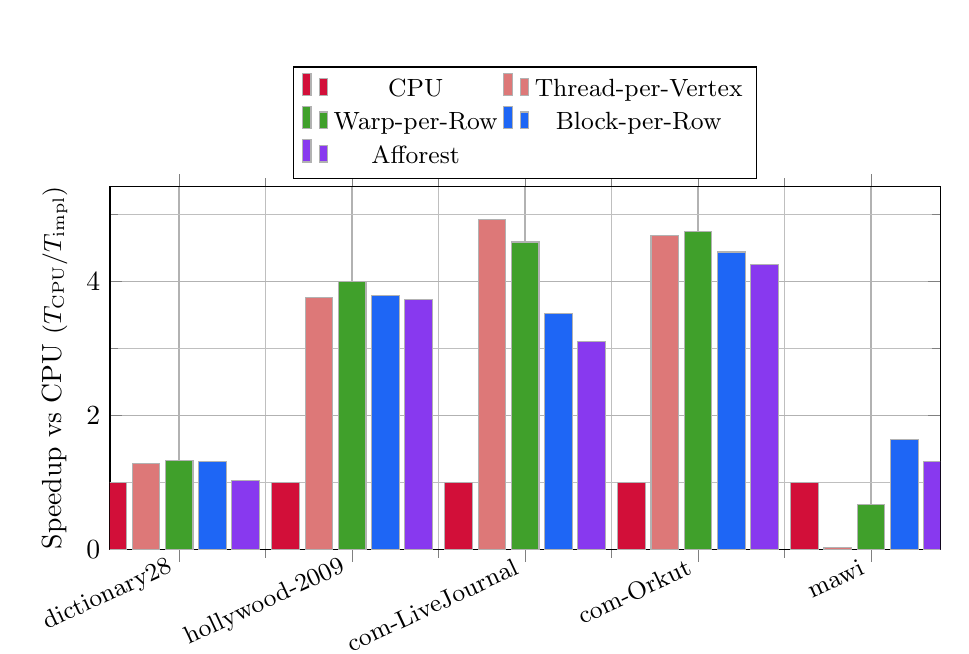
\begin{tikzpicture}
\begin{axis}[
    ybar,
    bar width=10pt,
    width=\linewidth,
    height=6.2cm,
    ymin=0,
    ylabel={Speedup vs CPU \small($T_{\mathrm{CPU}}/T_{\mathrm{impl}}$)\normalsize},
    symbolic x coords={dictionary28,hollywood-2009,com-LiveJournal,com-Orkut,mawi},
    xtick=data,
    x tick label style={rotate=25,anchor=east,font=\small},
    legend style={at={(0.5,1.02)},anchor=south,legend columns=2,font=\small},
    grid=both,
    minor tick num=1,
    major grid style={line width=0.5pt,draw=gray!60},
    minor grid style={line width=0.4pt,draw=gray!50},
]
% Baseline line at 1.0 (CPU)
\addplot+[mark=none,domain=0:1,fill=cpu,draw=black!30] coordinates {(dictionary28,1) (hollywood-2009,1) (com-LiveJournal,1) (com-Orkut,1) (mawi,1)};

\addplot+[fill=tpv,draw=black!30]      coordinates {(dictionary28,1.29) (hollywood-2009,3.76) (com-LiveJournal,4.93) (com-Orkut,4.68) (mawi,0.04)};
\addplot+[fill=warp,draw=black!30]     coordinates {(dictionary28,1.33) (hollywood-2009,4.00) (com-LiveJournal,4.59) (com-Orkut,4.74) (mawi,0.68)};
\addplot+[fill=block,draw=black!30]    coordinates {(dictionary28,1.31) (hollywood-2009,3.79) (com-LiveJournal,3.53) (com-Orkut,4.44) (mawi,1.65)};
\addplot+[fill=afforest,draw=black!30] coordinates {(dictionary28,1.03) (hollywood-2009,3.73) (com-LiveJournal,3.10) (com-Orkut,4.26) (mawi,1.32)};

\legend{CPU, Thread-per-Vertex,Warp-per-Row,Block-per-Row,Afforest}
\end{axis}
\end{tikzpicture}
\caption{Speedup relative to the sequential CPU baseline (higher is better).}
\label{fig:speedup}
\end{figure}

\begin{figure}[H]
\centering
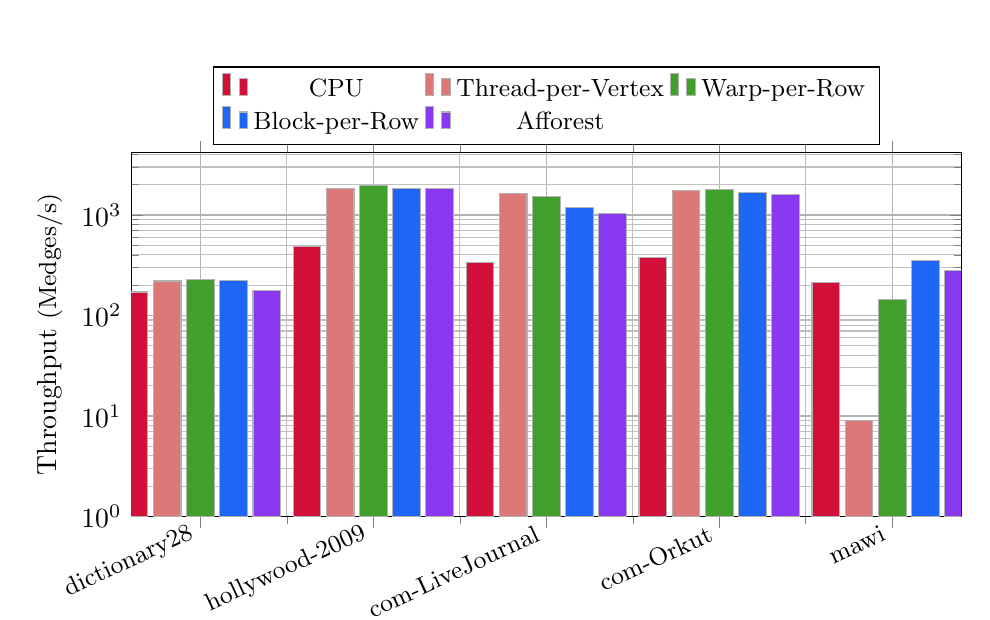
\begin{tikzpicture}
\begin{axis}[
    ybar,
    bar width=10pt,
    width=\linewidth,
    height=6.2cm,
    ymode=log,
    ymin=1,
    ylabel={Throughput \small(Medges/s)\normalsize},
    symbolic x coords={dictionary28,hollywood-2009,com-LiveJournal,com-Orkut,mawi},
    xtick=data,
    x tick label style={rotate=25,anchor=east,font=\small},
    legend style={at={(0.5,1.02)},anchor=south,legend columns=3,font=\small},
    grid=both,
    minor tick num=1,
    major grid style={line width=0.5pt,draw=gray!60},
    minor grid style={line width=0.4pt,draw=gray!50},
]
% CPU
\addplot+[fill=cpu,draw=black!30]      coordinates {(dictionary28,171.12) (hollywood-2009,487.28) (com-LiveJournal,333.84) (com-Orkut,377.90) (mawi,212.88)};
% GPU variants
\addplot+[fill=tpv,draw=black!30]      coordinates {(dictionary28,220.22) (hollywood-2009,1830.94) (com-LiveJournal,1645.50) (com-Orkut,1766.44) (mawi,8.92)};
\addplot+[fill=warp,draw=black!30]     coordinates {(dictionary28,227.78) (hollywood-2009,1951.74) (com-LiveJournal,1531.00) (com-Orkut,1789.00) (mawi,145.32)};
\addplot+[fill=block,draw=black!30]    coordinates {(dictionary28,223.68) (hollywood-2009,1846.48) (com-LiveJournal,1178.48) (com-Orkut,1676.96) (mawi,350.50)};
\addplot+[fill=afforest,draw=black!30] coordinates {(dictionary28,177.08) (hollywood-2009,1818.36) (com-LiveJournal,1033.94) (com-Orkut,1608.10) (mawi,281.74)};

\legend{CPU,Thread-per-Vertex,Warp-per-Row,Block-per-Row,Afforest}
\end{axis}
\end{tikzpicture}
\caption{Throughput across datasets (log scale). Social graphs achieve up to $\sim 2 \times 10^3$ Medges/s; MAWI exposes poor mapping choices, with Thread-per-Vertex collapsing below 10 Medges/s.}
\label{fig:throughput}
\end{figure}

\begin{figure}[H]
\centering
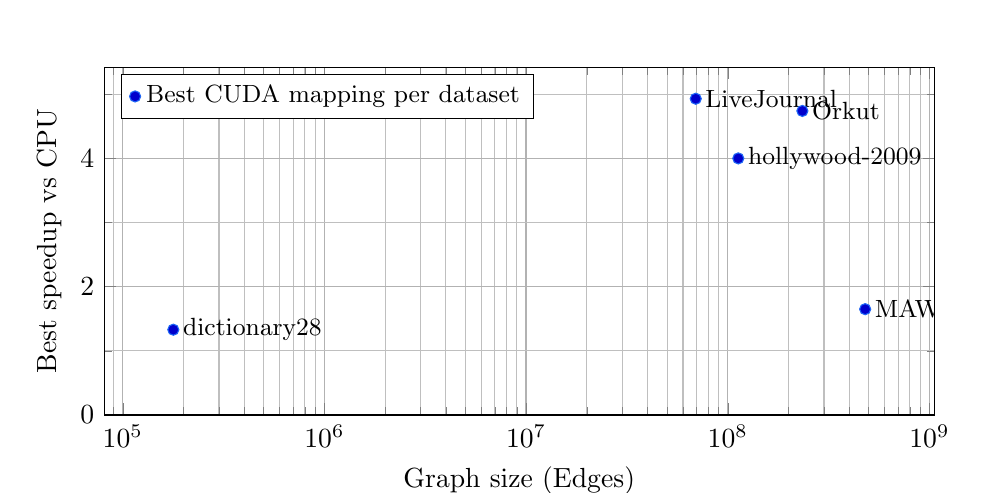
\begin{tikzpicture}
\begin{axis}[
    width=\linewidth,
    height=6.0cm,
    xmode=log,
    ymin=0,
    ylabel={Best speedup vs CPU},
    xlabel={Graph size (Edges)},
    grid=both,
    minor tick num=1,
    major grid style={line width=0.5pt,draw=gray!60},
    minor grid style={line width=0.4pt,draw=gray!50},
    legend style={at={(0.02,0.98)},anchor=north west,font=\small},
]
\addplot+[
    only marks,
    mark=*,
    draw=block,
    fill=block,
] coordinates {
    (178076,1.33)         % dictionary28 (best: Warp-per-Row)
    (112751422,4.00)      % hollywood-2009 (best: Warp-per-Row)
    (69362378,4.93)       % com-LiveJournal (best: Thread-per-Vertex)
    (234370166,4.74)      % com-Orkut (best: Warp-per-Row)
    (480047890,1.65)      % mawi (best: Block-per-Row)
};

% Add labels near points
\node[font=\small,anchor=west] at (axis cs:178076,1.33) {dictionary28};
\node[font=\small,anchor=west] at (axis cs:69362378,4.93) {LiveJournal};
\node[font=\small,anchor=west] at (axis cs:112751422,4.00) {hollywood-2009};
\node[font=\small,anchor=west] at (axis cs:234370166,4.74) {Orkut};
\node[font=\small,anchor=west] at (axis cs:480047890,1.65) {MAWI};

\legend{Best CUDA mapping per dataset}
\end{axis}
\end{tikzpicture}
\caption{Best observed speedup vs graph size. Small graphs are overhead-dominated; social graphs benefit most; extremely low-degree massive graphs (MAWI) limit GPU gains.}
\label{fig:size_vs_speedup}
\end{figure}

\section{Analysis and Discussion}
The results demonstrate that \textbf{GPU performance for connected components is highly workload-dependent}.
\begin{itemize}
	\item\textbf{Degree distribution matters}: Graphs with higher average degree and more uniform structure
	(e.g., social networks with avg degree 17–99) benefit the most from GPU parallelism. The correlation between
	average degree and speedup is evident in Table~\ref{tab:datasets} and Figure~\ref{fig:size_vs_speedup}.
	
	\item\textbf{Mapping choice is critical}: \textbf{Warp per row} consistently provides robust performance
	across most datasets by balancing parallelism and overhead. \textbf{Thread per vertex} is fragile and
	catastrophically fails on extremely low-degree graphs (MAWI: 0.04× speedup).
	
	\item\textbf{Overheads dominate small workloads}: For small graphs, GPU kernel launch and synchronization
	costs outweigh any parallelism benefits, as shown in Figure~\ref{fig:speedup} where dictionary28 achieves
	minimal speedup.
	
	\item\textbf{Low-degree massive graphs remain challenging}: \emph{MAWI} highlights the limits of GPU
	acceleration when computation per vertex is insufficient to hide memory latency and synchronization costs.
	With an average degree of only 2.1, there is simply not enough parallel work per vertex to justify GPU
	execution for naïve mappings.
\end{itemize}

These observations mirror known challenges in GPU graph analytics: maximizing useful work per thread and
minimizing divergence are essential for performance.

\section{Conclusions}
This work evaluated multiple CUDA-based connected components implementations on a single GPU. For medium and large
social graphs with moderate-to-high average degree, GPU acceleration achieves substantial speedups over a sequential
CPU baseline, with peak throughput \textbf{exceeding 1.9 billion edges per second}. However, performance varies
widely across datasets and kernel mappings. Simple GPU strategies fail catastrophically on extremely low-degree or
small graphs, while more cooperative mappings such as \textbf{warp per row} and \textbf{block per row} provide
better robustness.

Overall, GPUs are a powerful platform for connected components, but achieving high performance requires careful
consideration of graph structure—particularly average vertex degree—and execution mapping.

\section{Future Work}
Potential directions for further improvement include:
\begin{itemize}
	\item \textbf{Convergence analysis}: Instrument the code to track and report the number of iterations required
	for convergence across different implementations and graph structures. This would help explain performance
	differences beyond just throughput.
	
	\item \textbf{Graph reordering}: Implement degree-sorted vertex reordering to improve locality and reduce
	divergence. High-degree vertices could be processed first to accelerate component merging.
	
	\item \textbf{Hybrid CPU–GPU approaches}: For irregular or low-degree graphs like MAWI, explore strategies
	that partition the graph based on degree distribution, processing low-degree vertices on CPU and high-degree
	vertices on GPU.
	
	\item \textbf{Multi-GPU scaling}: Investigate graph partitioning strategies for multi-GPU execution with
	overlap of computation and inter-GPU communication.
	
	\item \textbf{Memory bandwidth profiling}: Add fine-grained profiling using NVIDIA Nsight Compute to separate
	computation time, memory transfer time, and synchronization overhead. This would identify bottlenecks more
	precisely.
	
	\item \textbf{Alternative algorithms}: Compare against BFS-based connected components and Shiloach-Vishkin
	algorithms to understand whether union-find is optimal for GPU execution.
	
	\item \textbf{Dynamic parallelism}: For graphs with highly variable degree distribution, explore CUDA dynamic
	parallelism to adaptively select thread-per-vertex vs warp-per-row vs block-per-row based on runtime degree
	analysis.
\end{itemize}

\noindent\textbf{Code Availability:} Source code and benchmark results are available at:\\
\url{https://github.com/dimgerasimou/pds-hw3-cuda-connected-components}.

\end{document}
